
%First page for bachelor thesis at LIACS: bachelorpage.tex
%Needed: unique serial number + date; name thesis and author
%Version September 2010

%Usage: 
%  latex bachelorpage.tex
%  dvips -Ppdf bachelorpage.dvi
%  ps2pdf bachelorpage.ps
%Needed: file ullogo.eps for the university logo
%
%  concatenate bachelorpage.pdf with yourthesis.pdf to yourfinalthesis.pdf by means of
%  gs -q -sPAPERSIZE=a4 -dNOPAUSE -dBATCH -sDEVICE=pdfwrite -sOutputFile=yourfinalthesis.pdf bachelorpage.pdf yourthesis.pdf

\documentclass[12pt]{article}


\setlength{\textheight}{24.7cm}
\setlength{\textwidth}{16cm}
\setlength{\unitlength}{1mm}
\setlength{\topskip}{1truecm}
\topmargin 280mm \advance \topmargin -\textheight
\divide \topmargin by 2 \advance \topmargin -1in
\headheight 0pt \headsep 0pt
\leftmargin 210mm \advance \leftmargin -\textwidth
\divide \leftmargin by 2 \advance \leftmargin -1in
\oddsidemargin \leftmargin \evensidemargin \leftmargin
\parindent=0pt
\frenchspacing
\usepackage{graphicx}

\usepackage{algorithm2e}
\usepackage{listings}

\usepackage{biblatex}
\bibliography{thesis}


\begin{document}

%No page number
\thispagestyle{empty}

\begin{large}

%Logo Leiden University
\vspace*{4mm}\hspace*{-13mm}
\includegraphics{ullogo.eps}

\vspace*{-3.5cm}

\sf 

%Ask for a unique serial number! And the date ...
\hspace*{2.5cm}Internal Report 2013--number \hfill June 2013

\vspace*{5mm}

\begin{Huge}
\hspace*{2.5cm}\textbf{Universiteit Leiden}

\vspace*{8mm}

\hspace*{2.5cm}\textbf{Opleiding Informatica \& Economie}
\end{Huge}

\vspace*{4.5cm}

\begin{Large}
%Here your title
\hfill Datamining 

\vspace*{3mm}

\hfill with Physiological Data

\vspace*{3mm}

\hfill from Multiple Sensor Systems

\vspace*{4cm}

%Here your name
\hfill Michiel Vos

\end{Large}

\vspace*{3.5cm}

\hspace*{2.5cm}BACHELOR THESIS

\vspace*{1mm}

\hspace*{2.5cm}Leiden Institute of Advanced Computer Science (LIACS)\\
\hspace*{2.5cm}Leiden University\\
\hspace*{2.5cm}Niels Bohrweg 1\\
\hspace*{2.5cm}2333 CA Leiden\\
\hspace*{2.5cm}The Netherlands\\
\hspace*{2.5mm}\ 

\end{large}

\vspace*{-24.3cm}
\begin{tabular}{p{1.5cm}|l}
\ &\ \\\ &\ \\\ &\ \\\ &\ \\
\ &\ \\\ &\ \\\ &\ \\\ &\ \\
\ &\ \\\ &\ \\\ &\ \\\ &\ \\
\ &\ \\\ &\ \\\ &\ \\\ &\ \\
\ &\ \\\ &\ \\\ &\ \\\ &\ \\
\ &\ \\\ &\ \\\ &\ \\\ &\ \\
\ &\ \\\ &\ \\\ &\ \\\ &\ \\
\ &\ \\\ &\ \\\ &\ \\\ &\ \\
\ &\ \\\ &\ \\\ &\ \\\ &\ \\
\ &\ \\\ &\ \\\ &\ \\\ &\ \\
\ &\ \\\ &\ \\\ &\ \\\ &\ \\
\ &\ \\\ &\ \\\ &\ \\
\end{tabular}

\begin{abstract}
This is the abstract

\end{abstract}


\tableofcontents

\section{Introduction}
	\subsection{Preface}
		This bachelor thesis is part of the track Informatica \& Economie at the Universiteit Leiden. In the first semester I followed the course Data Mining\footnote{A definition of data mining is the process of discovering patterns in data, by analyzing the data automatically\cite{datamining}.} lectured by Arno Knobbe and got an 8,5 as grade. I became interested in the subject and wanted to do my bachelor project on one of the projects there were offered. I like to sport and do it at least four times a week. I football at svKMD in the first team and cycling at WTOS, a student club. During cycling I'm using a Garmin Edge 705 to keep track of my heart rate, speed, average speed and have a spreadsheet with the amount of kilometers per route. In this project I have combined sport and tracking which resulted in a lot of fun. Thanks Ricardo Cachucho for assisting me and Arno Knobbe for helping and providing the project.

	\subsection{Motivation}
		Actions have consequences and some are clear for us humans and others aren't. When something is happening directly after the action and it's consistent, it's easy recognizable as cause-effect. The longer the delay between the cause and effect the less certain we're about the correlation, but we can still be convinced about our guess about the causality if the pattern happens repeatedly. For example drinking coffee before sleep and laying awake in bed later. Still it is difficult to prove because all other variables that could interupt sleep should be fixed while experimenting, which is not possible. We could use data mining to help us find causalities about sleep and actions we do during the day. It would give insight how things works and help us improve our life style and quality. Maybe it's in the future possible to explain health complains automatically.

	\subsection{Problem Statement}
		Our live is producing so much data, it's not possible to imagine. But still, every bit more data gathered could provide interesting inside. We are trying to gather as much as possible data, within the trivial boundaries in research. Tracking your live must be convenient and should not disturb live and it's producing data. Setting up such experiment has all kind of practical problems. The raw data is not useable for any data mining algorithm, because the source and format are different. There is much to be done to transform it in a clean dataset, and even this clean dataset can be transformed and restructured to get an extended or derivative dataset. 

		Then there is a discussion which data mining technique can be used. 


			
		Time series, labeled, target

		How to deal with different data systems, collecting the data and working with problems, reorganize the data to get a nice dataset (useable for Data mining), use Data Mining techniques.

		what: self-tracking routines
		How: sensor systems
		Challenge: data integration \& Modeling
		goal: 1 dataset \& model
%	\subsection{Motivation}
%		Arno description + personal motivation
%		find correlation between 'pains' and how you lived you day / night. 
%		Try to automaticly analyze the day/night.

	\subsection{Outline}
		It's important to explain which systems are being used, what the data means and how the data looks like. Next section there is a comparison between the two physiological devices, what was really useful to learn the devices. The data collection is the most important part of the thesis, because it's explaining how everything was set up and done to get the provided dataset. - Modeling - Conclusions 

		In the Sensor System section the hardware is explained, what the sensors does, what the applications are and how it works. 
		In the experiments section describes useful derivative data, a comparison between the two physiological devices and the experiment to combine all three devices to a good dataset.
		Modeling: I made a dataset of 15 days with all kind of features. Set the deep sleep as target attribute and use WeKa to make a model, with a discussion why deep sleep as target, how the algorithm works and hopefully some insights of the model. 


\section{Sensor systems}
	\label{sec:sensorsystems}
	\subsection{BioHarness}
			The Zephyr Bioharness 3\cite{bioharness} is a physiolocigal monitoring device, which is attached to a strap on the chest. There are several practical uses for this device.
			\begin{itemize}
				\item Remote patient monitoring. Medical patients who need health care but want to live at home, in combination with ZephyrLIFE \texttrademark \cite{bhpatients}.
				\item Sporters who would like to track their progress.
				\item For coaches to find out who is tired and up for substitution during a match \cite{bhsport}.
				\item In 2010 Chilean mineworkers who were trapped underground were remotedly monitored which resulted in a better rescue order and better health care when the miners were again above ground. \cite{chile}
				\item Researchers who could use the data.
			\end{itemize}

			The device has an internal storage for more than 500 hours logging and the battery's life cycle is up to 35 hours. The device can be connected to a pc with a USB cable, to transfer data and to recharge the battery. The following logs could be produced: general log, summary log, summary and waveform log and the event log. 
			It takes around 1-6 minutes per hour of data to download the log files from the device to a computer. \cite{bhdatasheet} The data is stored in a folder per session\footnote{A period from which the device is on till it's turned off is called a session.} and within the folder different CSV\footnote{CSV stands for Comma-Separated Values and such file can be opend with e.g. Microsoft Excel. Zypher also provides scripts to convert CSV files to Matlab files.} and DaDisp\footnote{``DADiSP scientific computing and data visualization software that combines the power of programming with the simplicity of a spreadsheet''\cite{dadisp}.} files. The sampling frequency of the CSV files differs from the sampling frequency of the sensors. Most logs are sampled at \SI{1}{\hertz}.
			The price is \$ 472.
		
			The accelerometer measures the physical acceleration of the user in the x-, y- and z-axis.. $m/s^2$ is a unit of $g$. The sampling rate is 100 Hz\footnote{Hz stands for hertz and is defined as the number of cycles per second.}. The range is from $-16g$ to $+16g$ for each axis. The acceleration magnitude is $\sqrt{(\Delta X)^2+(\Delta Y)^2+(\Delta Z)^2}$.

			The breathing sensor measures the pressure of the chest to the sensor. If the pressure is above a certain threshold it will count as a breath taken. The breath rate is the amount of breaths taken in a minute. The sampling frequency is 25 Hz and the ranges is from 0 to 120.

			The electrocardiography\cite{ECG} (ECG) sensor measures the electrical activity of the heart. See Figure~\ref{fig:ecg} for a graph of the results an ECG produces. The sampling frequency is 1000 Hz.

			\begin{figure}[h]
				\centering
					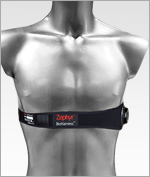
\includegraphics[scale=2.0]{bh.jpg}
					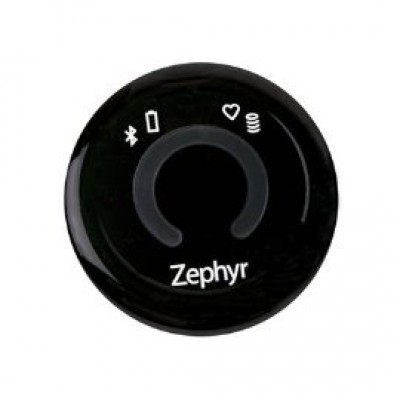
\includegraphics[scale=0.25]{bhclose.jpg}
					
					\caption{The BioHarness}

			\end{figure}

			\begin{figure}[h]
				\centering
					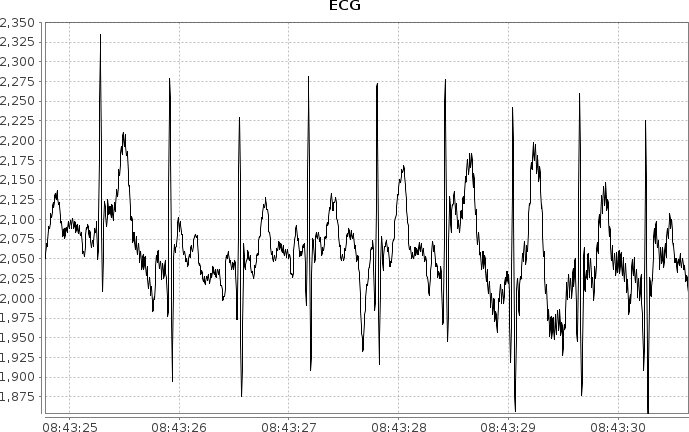
\includegraphics[scale=0.5]{ecg.png}
					
				\caption{A graph of 5 seconds of ECG data}
				\label{fig:ecg}

			\end{figure}
			
			% R-R: 250 - 1500 ms, 25 Hz

			% heart rate, R-R interval, breathing rate, ECG, postsure, activity, acceleration

			%The data in stored in a csv file and is an 2D array, for every session a csv file. it's resampled to \SI{1}{Hertz}.
		%Timestamp,HR,BR,Temp,Posture,Activity,Acceleration,Battery,BRAmplitude,ECGAmplitude,ECGNoise,XMin,XPeak,YMin,YPeak,ZMin,ZPeak
	\subsection{Beddit}
		%\subsubsection{General}
		The Beddit Sleep Tracker is placed next to a bed and is connected with a sensor between the sheets and the mattress. The makers of Beddit think sleep is important, because a human is sleeping one third of his live. Better sleep results in a better life quality. Why not measure it to help improve our sleep quality? The sensor is about \SI{70}{\centi\metre} long and \SI{4}{\centi\metre} wide, so it's possible it will not cover the whole bed. 
			The price is \EUR{395}.

			The ballistocardiogram (BCG) measures (micro)movements of the body.\cite{beddit}
			BCG is convenient in use, because you won't notice it's measuring, but the disadvantage compared to ECG it's not only measuring cardiac activity, but also body movements, like tossing and turning, which could also be an advantage.\cite{bcg} The sampling frequency is \SI{140}{\hertz}. The devices also measure the room temperature (\SI{}{\celsius}), ambient noise level (\SI{}{\decibel}) and brightness (\SI{}{\lux}), once per 5 minutes\cite{bedditapi}.

			The data is stored in two JSON\footnote{JSON stands for JavaScript Object Notation and is a format to exchange data between different software environments.\cite{json}} files per session.

			\begin{figure}[h]
				\centering
					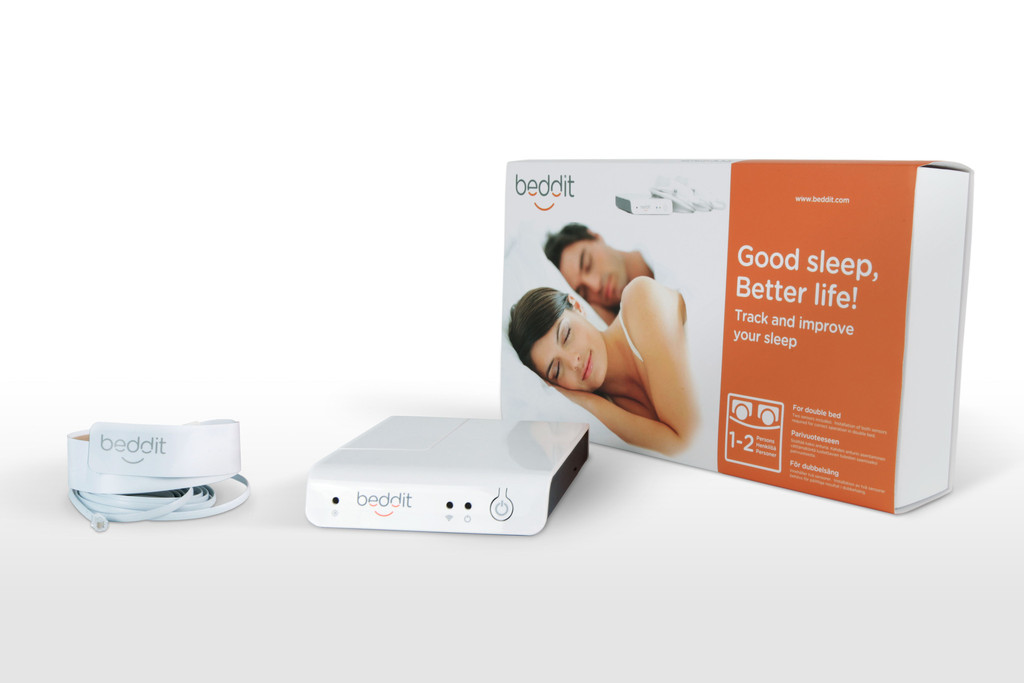
\includegraphics[scale=0.25]{beddit.jpg}
					
					\caption{The Beddit sensor and the device\cite{beddit}}

			\end{figure}

		%\subsubsection{Description}
		%		Respiration, presence, ihr, actigram, noise, luminosity, temperature, sleep stages, 
		% \subsubsection{Format}
		%	Per day there are two JSON files.
		%	\lstset { 
		%		basicstyle = \footnotesize,
		%		tabsize = 2
		%	}
			%\lstinputlisting[caption=Sleep]{beddit.listing}
			%\lstinputlisting[caption=Results]{beddit2.listing}


	\subsection{Openbeacon}
		%\subsubsection{General}
	RFID stands for Radio-frequency identification and is a technology to communicate wireless between tags. The OpenBeacon Ethernet EasyReader PoE II (called OpenBeacon from now) can receive and send signals with those tags. See Figure~\ref{fig:openbeacon} for a picture of a tag and the device. There're two kind of tags, active and passive ones. Active tags are powered by a battery and can broadcast their signal. Passive tags don't have batteries and are powered by the energy received wireless from the OpenBeacon, but only when they're in range. The tags of the Openbeacon are active tags and can also communicate with each other. The OpenBeacon Ethernet EasyReader PoE II can identify RFID tags and edges between the tags. Each tag has it's own ID and each edge has a power level. It takes the Openbeacon a few seconds to identify the edges. The price of 100 RFID tags is \EUR{1575,75} an the EasyReader costs \EUR{184,87} euro. RFID tags have a lot of applications, like: theft protection on clothing, as access key pas to enter buildings, track and trace of goods while transporting and social experiments\cite{2008arXiv0811.4170B}. The OpenBeacon produces JSON output.


			\begin{figure}[h]
				\label{fig:openbeacon}
				\centering
					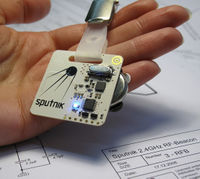
\includegraphics[scale=0.5]{tag.jpg}
					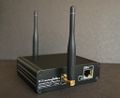
\includegraphics[scale=1.0]{reader.jpg}
					
					\caption{A tag for the OpenBeacon\cite{openbeacon} and the OpenBeacon Reader}

			\end{figure}

		%\subsubsection{Description}
		%timestamp, tag1, tag2, power level

		%\subsubsection{Format}
		%The data is stored in a MongoDB in the following format:
		%Tags: ID, Timestamp
		%Edges: Timestamp, Tag1, Tag2

\section{Experiments}
	\subsection{Data description}
	\label{sec:datadescription}
		\subsubsection{BioHarness}
		From the data produced by the sensors more data can be derived. For the experiments the general log is used, because it has the most interesting variables and a lot preprocessing is already done. The heart rate is the amount of beats per minute and can be derived from the ECG. In the ECG graph (See Figure~\ref{fig:ecg}) a pattern is visible, also called a cycle. Each cycle is one heartbeat. 
			The accelerometer measures the acceleration magnitude. The peak acceleration is logged in the general log.
			The activity level is derived from the accelerometer and is expressed in terms of VMU\footnote{Vector Magnitude Units} (g).
			The force and direction of the gravity is known and the BioHarness is worn at the chest, so it's possible to calculate the posture of the user. The range is 180 degrees. \SI{0}{\celsius} is vertical and \SI{180}{\celsius} is inverted.
			Breath rate is derived from the breath sensor. The relative slow transfer rate from the device to the pc could be explained by the ?calculating/generating/computing? of the new data. The sampling frequency of the general log is \SI{1}{\hertz}.
		\subsubsection{Beddit}
		\label{sec:datadescriptionbeddit}
		The data from the sensors is being transferred via wifi or cable to the web servers of Beddit, almost realtime. The servers are analyzing the data and extracting the heart rate, respiration\footnote{Beddit uses the term respiration for breathing.} and the activity from the BCG. When all data is received of the night, the servers are going to analyze it and will compute the sleep stages, sleep efficiency\footnote{Relative time sleeping compared to time in bed}, average heart rata, average noise level and stress level. The stages are ``Away'', ``Wake'', ``Light sleep'', ``Deep sleep'', ``REM''\footnote{REM stands for Rapid Eye movements, it's a very light sleep and dreaming is possible in this stage.} and ``Missing''. How Beddit computed these stages is not explained, but they probably use the heart rate and the binary actigram. Beddit doesn't use a constant sampling frequency. For the respiration and the instant heart rate there is a record for every beat, with the BPM computed from two single heart beats and the timestamp in seconds since the start of the session. Presence has a record for every second the presence is changing and a 0 if the user is not in bed and a 1 if the user is in bed. The binary actigram has a record for every second there is a movement above a certain threshold. The minutely actigram has for every minute a value with the amount of movements occurred. The temperature, ambient noise level and brightness have a record every 5 minutes with the date and time in ISO 8601\footnote{Example 2013-05-14T19:04\cite{iso8601}} format in locale time and their values, respectively celsius, decibel and lux.

		\subsubsection{OpenBeacon}
			The Openbeacon produces JSON and is stored in a NoSQL\footnote{A NoSQL database is the counterpart of a relational database. One argument to use it is because it's more flexible.} database MongoDB. The collections of the database can be exported as csv files.
			There are two collections. The collection tags, within documents with the format tag ID, timestamp\footnote{Amount of seconds since 00:00:00 GMT January 1, 1970 (the UNIX epoch)} . For every second the OpenBeacon sees a tag, a document will be added.
			The second collection called edges. For every second the OpenBeacon sees an edge between two tags, there will be one document added with the format ID of tag 1, ID of tag 2, power level and timestamp.
			The higher the power level the closer the tags are from each other. The power level can not be expressed in terms of distance, because there are other things that could interfere the power level. For example walls and other communication on the \SI{2.4}{\giga\hertz} frequency.
	\subsection{Beddit versus BioHarness}
		\label{sec:bvsb}
		\subsubsection{Comparison}
			The first experiment is a comparison between the Beddit and the BioHarness. It's a good assignment to get to know the devices and the data. The two devices have overlapping features like the heart rate, breath rate and activity level. It would be a good test to see if they measure the same thing. 
			Beddit does not have a constant sampling frequency. After every heartbeat the bpm is computed between the heartbeat and the previous heartbeat. The value is notated with the amount of seconds since the session. For every heartbeat, the associated minute and the heart rate is summed up with all the other heartbeat heart rates, and divided by the amount of heartbeats in the specific minute. This results in an average heart rate per minute. The respiration rate is also summed up, but doesn't needs to be divided, because it's the amount of breaths taken.
			The BioHarness heart rate, breath rate and activity calculations are done the same. The difference is the Bioharness has a constant sampling frequency from \SI{1}{\hertz}. 
			The Beddit binary actigram has already one record per minute, it just needs to be copied. It's not the same as the BioHarness activity, so it would be good to standardize\footnote{Standardization makes it easier to compare values with different scales} the BioHarness activity and the Beddit binary actigram.
			\begin{figure}[h]
				\begin{equation}
					\label{eq:standardize}
					\mu = \frac{ \sum\limits_{i=1}^n y_i } { n }
				\end{equation}
				\begin{equation}
					D_i = (X_i - \mu)^2
				\end{equation}
				\begin{equation}
					\sigma = \sqrt{ \frac{ \sum\limits_{i=1}^n D_i } { n } }
				\end{equation}
				\begin{equation}
					standardized\ value_i = \frac{ y_i - \bar{y} } { \mu }
				\end{equation}
				\caption{Standardization method\cite{statistics}}
			\end{figure}

			Both devices were used for one night. The sampling frequency is \SI{16.67}{\milli\hertz} (every one minute). Minutes with missing data are removed. Section \ref{sec:datacollection} explains more about the setup and how to bundle the data. Sleeping with the BioHarness is possible when laying on the back. Sleeping on the left side is not comfortable. The tool QUICKIE\footnote{QUICKY stands for Quick User Interface for Convolution Kernel-Involving Experiments and is being made and used by the Data Minig Group of Liacs, but is not yet published.} is used to visualize the data and find the correlations.

		\subsubsection{Results}
			
			\begin{figure}[h]
				\centering
					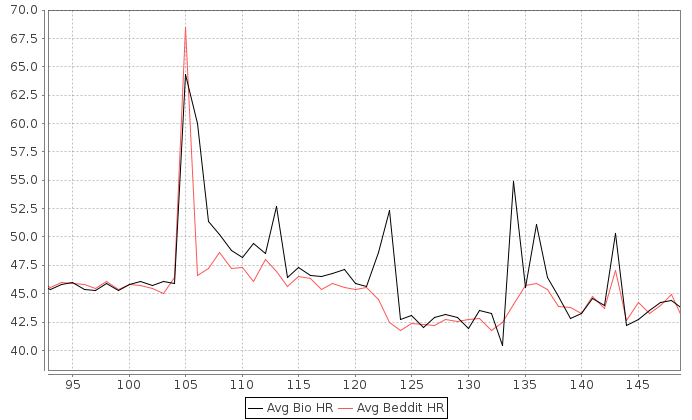
\includegraphics[scale=0.5]{avgbiovsavgbeddit.png}
					
				\caption{Part of the plot of the heart rate}
				\label{fig:avgbiovsavgbeddit}

			\end{figure}

			The lines in Figure~\ref{fig:avgbiovsavgbeddit} are not exactly the same, but do have the same pattern. The correlation is 0.61. The low correlation could be explained by lag in measurements or one (or both) devices doesn't measure it correct. Moving average is a technique to smooth the lines. If width 7 is used, then it means a value on the new computed line is composed from the current and the previous 6 minutes of the old line. If moving average is applied to both lines, the correlation of the heart rates will be 0.98.\
						
			\begin{figure}[h]
				\centering
					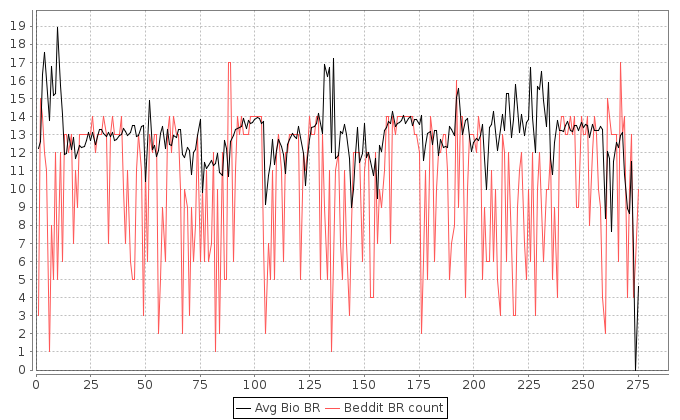
\includegraphics[scale=0.5]{vsbr.png}
					
				\caption{Plot of the breath rate}
				\label{fig:vsbr}

			\end{figure}

			The lines in Figure~\ref{fig:vsbr} are different. The correlation is 0.12. When moving average (width 10) is used the correlation is still 0.71. There is something wrong or the devices are measuring something else. The correlation of the standardized values is 0.26. 
						
			\begin{figure}[h]
				\centering
					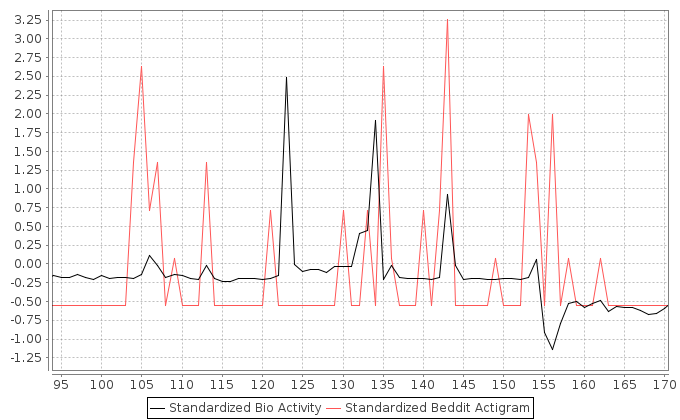
\includegraphics[scale=0.5]{vsactivity.png}
					
				\caption{Part of the plot of the activity}
				\label{fig:vsactivity}

			\end{figure}
			The Beddit actigram and the BioHarness activity are something different, so standardization is used. Figure~\ref{fig:vsactivity} shows some similarities, but the correlation is still low (0.26). Moving average doesn't help to improve the correlation.

			The heart rates of the Bioharness and the Beddit could be merged to one variable. The BioHarness breath rate and the Beddit respiration rate is totally different. The lines of the activity are a bit like each other, but the correlation of the activity is low and by far not good enough to merge them into one variable.

	\subsection{Data collection}
		\label{sec:datacollection}
		\paragraph{Beddit}
			The sensor is placed on my bed and connected with the device. The device is connected to the internet. Beddit starts measuring from 21:30 till 11:00 the next day. After all the measuring I've downloaded for every night two JSON files with the API of Beddit\cite{bedditapi}. After the computing of the data I received an email and I visited the website to see if everything is logged alright.
		\paragraph{BioHarness}
			When I wake up, I start my PC and the BioHarness Log Downloader. After about 40 minutes I've took a shower and had breakfast, the Log Downloader is ready. I put the strap on my chest with the device and turn it on. After sport I take a shower and put it off and after shower again on. The device is water resistance up to one meter, but it takes a while for the strap to get dry. Right before I go to bed I connect the device to the PC so it's recharged again the next day. I'm missing a few minutes data every day because of the Log Downloader and the showering. 
		\paragraph{Openbeacon}
			In the experiment the OpenBeacon is used as a localization tool. The location of the user could explain some behaviour during the day, which can explain behaviour during the night. At first there were two OpenBeacon devices available, one for the ground floor and one for the second floor. It covered the whole house, but unfortunately one device stopped working. The working device were set up at the ground floor and several tags at the following places: dining room, toilet ground floor, kitchen, living room, hall first floor, toilet first floor. I were wearing also a tag. If there was an edge between my tag and the tag dining room, my location was the dining room for example. The OpenBeacon was always on, but the script to capture the JSON output and storage it in the MongoDB not. After waking up I started my laptop and the script. I took my tag with me, except in the shower where it was put at on a cabinet at the hall first floor. When I left the house the script was stopped and when I came back home I started the script right away. There are a few minutes missing data every day. For example, I'm late back home from sport and I went to bed, but not before changing clothes, brushing teeth, unpacking my sport bag etc, without wearing my tag, because the script was not running. Of course the script is stopped before going to bed.
			
			A few locations were I was at a certain time are known, but more locations could be extracted with some tricks. See Figure~\ref{fig:decisiontree} for the decision tree.

				\begin{figure}[h!]
					\begin{tikzpicture}[
% Gates and symbols style
    and/.style={and gate US,thick,draw,fill=red!60,rotate=90,
		anchor=east,xshift=-1mm},
    or/.style={or gate US,thick,draw,fill=blue!60,rotate=90,
		anchor=east,xshift=-1mm},
    be/.style={circle,thick,draw,fill=green!60,anchor=north,
		minimum width=0.7cm},
    tr/.style={buffer gate US,thick,draw,fill=purple!60,rotate=90,
		anchor=east,minimum width=0.8cm},
% Label style
    label distance=3mm,
    every label/.style={blue},
% Event style
    event/.style={rectangle,thick,draw,fill=yellow!20,text width=2cm,
		text centered,font=\sffamily,anchor=north},
% Children and edges style
    edge from parent/.style={very thick,draw=black!70},
    edge from parent path={(\tikzparentnode.south) -- ++(0,-1.05cm)
			-| (\tikzchildnode.north)},
    level 1/.style={sibling distance=7cm,level distance=1.4cm,
			growth parent anchor=south,nodes=event},
    level 2/.style={sibling distance=7cm},
    level 3/.style={sibling distance=6cm},
    level 4/.style={sibling distance=3cm}
%%  For compatability with PGF CVS add the absolute option:
%   absolute
    ]
%% Draw events and edges
    \node (g1) [event] {No flow to receiver}
	     child{node (g2) {No flow from Component B}   
	     	child {node (g3) {No flow into Component B}
	     	   child {node (g4) {No flow from Component A1}
	     	      child {node (t1) {No flow from source1}}
	     	      child {node (b2) {Component A1 blocks flow}}
			}
	     	   child {node (g5) {No flow from Component A2}
	     	      child {node (t2) {No flow from source2}}
	     	      child {node (b3) {Component A2 blocks flow}}
			}
		   }
	     	child {node (b1) {Component B blocks flow}}
		};
%% Place gates and other symbols
%% In the CVS version of PGF labels are placed differently than in PGF 2.0
%% To render them correctly replace '-20' with 'right' and add the 'absolute'
%% option to the tikzpicture environment. The absolute option makes the 
%% node labels ignore the rotation of the parent node. 
   \node [or]	at (g2.south)	[label=-20:G02]	{};
   \node [and]	at (g3.south)	[label=-20:G03]	{};
   \node [or]	at (g4.south)	[label=-20:G04]	{};
   \node [or]	at (g5.south)	[label=-20:G05]	{};
   \node [be]	at (b1.south)	[label=below:B01]	{};
   \node [be]	at (b2.south)	[label=below:B02]	{};
   \node [be]	at (b3.south)	[label=below:B03]	{};
   \node [tr]	at (t1.south)	[label=below:T01]	{};
   \node [tr]	at (t2.south)	[label=below:T02]	{};
%% Draw system flow diagram
   \begin{scope}[xshift=-7.5cm,yshift=-5cm,very thick,
		node distance=1.6cm,on grid,>=stealth',
		block/.style={rectangle,draw,fill=cyan!20},
		comp/.style={circle,draw,fill=orange!40}]
   \node [block] (re)					{Receiver};
   \node [comp]	 (cb)	[above=of re]			{B}  edge [->] (re);
   \node [comp]	 (ca1)	[above=of cb,xshift=-0.8cm]	{A1} edge [->] (cb);
   \node [comp]	 (ca2)	[right=of ca1]			{A2} edge [->] (cb);
   \node [block] (s1)	[above=of ca1]		{Source1} edge [->] (ca1);
   \node [block] (s2)	[right=of s1]		{Source2} edge [->] (ca2);
   \end{scope}
\end{tikzpicture}

					\caption{A decision tree how to find more locations}
					\label{fig:decisiontree}
				\end{figure}

				Strange enough some tags were showing up which were not part of the tags of the OpenBeacon. These 'tags' were ignored.
				
	\subsection{Preprocessing}
		\label{sec:preprocessing}
		\subsubsection{From raw to a dataset}
			In this phase all the data is used and combined to have one structed dataset after the phase. The end result is a csv file. The sampling frequency is \SI{1}{\hertz}, which means for every second a row. The dataset begins at Wed 10 Apr 2013 08:43:01 AM CEST GMT+2 and ends at Thu 25 Apr 2013 08:52:35 AM CEST GMT+2. 
			
			%\pagebreak

\lstset{
	language=Python,
	numbers=left,
	numberstyle=\tiny,
	frame=tb,
	basicstyle=\small,
	tabsize=2,
}
\begin{lstlisting}[caption=Pseudocode]
// Initializing
data = []
begin = 10 April 2013 08:43:01
end = 25 April 2013 08:52:35
for every second from begin to end:
	data[second] = {}

// Reading
for every day:
	// Beddit
	beddit = readBedditFiles(day)
	for 'presence', 'respiration', 'ihr', 'sleep stage', 'noise',
		'luminosity', 'temperature', 'minutely actigram' as attribute:
		for every attribute in beddit as value:
			timestamp = convertToTimestamp(value)
			data[timestamp]['beddit' + attribute] = value

	?OR?

	for every presence in beddit:
		timestamp = convertTime(presence)
		data[timestamp]['beddit'] = presense
	for every respiration in beddit:
		timestamp = convertTime(respiration)
		// Amplitude, minToMin, maxToMax
		data[timestamp]['beddit_respiration'] = respiration
	for every ihr in beddit:
		timestamp = convertTime(ihr)
		// Instant heart rate
		data[timestamp]['beddit_ihr'] = ihr
	for every sleep stage in bddit:
		timestamp = convertToTimestamp(sleep stage)
		data[timestamp]['beddit sleep stage'] = sleep stage

	// BioHarness
	bioharness = readBioharnessFile(day)
	timestamp = getTime(bioharness)
	for every second in bioharness:
		for 'hr', 'br', 'activity', 'acceleration', 'posture',
			'BRAmplitude', 'ECGAmplitude', 'ECGNoise', 'XMin', 'XPeak',
			'YMin', 'YPeak', 'ZMin', 'ZPeak' as attribute:
			data[timestamp]['bioharness ' + attribute] = second[attribute]


	// OpenBeacon
		// set all locations 0
		for every second of the day
			for 'out', 'dining room', 'toilet ground floor', 'kitchen',
				'living room', 'toilet first floor', 'rest', 'bed' as location:
				data[timestamp][location] = 0

		openbeacon = readerOpenBeaconFile(day)
		for every second in openbeacon:
			timestamp = getTimestamp(second)
			// See Figure Decision Tree
			location = findLocation(openbeacon, data[timestamp])
			data[timestamp][location] = 1

// Writing csv file

writeHeader()
for every second in data:
	row = []

	// Copy OpenBeacon
	for 'out', 'dining room', 'toilet ground floor', 'kitchen',
		'living room', 'toilet first floor', 'rest', 'bed' as location:
		row[location] = data[second][location]

	// Copy Beddit respiration
	for 'amplitude', 'minToMin', 'maxToMax' as attribute:
		if 'beddit respiration ' + attribute in data[second]:
			row['beddit respiration ' + attribute] = 
				data[second]['beddit ' + attribute]
		else:
			row['beddit respiration ' + attribute] = 'null'

	// Copy rest of Beddit
	for 'ihr', 'sleep stage', 'noise', 'luminosity', 'temperature',
		'minutely actigram' as attribute:
		if 'beddit ' + attribute in data[second]:
			row['beddit ' + attribute in data[second] =
				data[second]['beddit ' + attribute]
		else:
			row['beddit ' + attribute in data[second] = 'null'

	// Copy BioHarness
	for 'hr', 'br', 'activity', 'acceleration', 'posture',
			'BRAmplitude', 'ECGAmplitude', 'ECGNoise', 'XMin', 'XPeak',
			'YMin', 'YPeak', 'ZMin', 'ZPeak' as attribute:
		if 'bioharness ' + attribute in data[second]:
			row['bioharness ' + attribute =
				data[second]['bioharness ' + attribute]
		else
			row['bioharness ' + attribute = 'null'

	// Write row
	writeRow(row)

	

\end{lstlisting}


			Most of the code is loops and more loops, calculating the right timestamp and copy data. 
			The Beddit API only give records of the sleep stage and timestamp, when the stage is changing. The gaps with missing values are filled in. See Figure~\ref{fig:missingvalues}. There are still a lot of missing values. For example the heart rate at night. It is possible to use methods to fill in the gaps, but it's better to provide a 'raw' dataset, with only the facts. When someone would like to use the data, the person can decide herself/himself the method or solution.
			\begin{figure}[h!]
			\[ 
				\left(
				\begin{array}{c}
				Away \\
				null \\
				null \\
				Wake \\
				null \\
				Light sleep \\
				Deep sleep \\
				null \\
				Light sleep \\
				null \\
				Wake \\
				Away \\
				null
				\end{array}
				\right)
				\to
				\left(
				\begin{array}{c}
				Away \\
				Away \\
				Away \\
				Wake \\
				Wake \\
				Light sleep \\
				Deep sleep \\
				Deep sleep \\
				Light sleep \\
				Light sleep \\
				Wake \\
				Away \\
				Away 
				\end{array}
				\right)
			\] 
			\caption{How the missing values are filled in of the sleep stages}
			\label{fig:missingvalues}
		\end{figure}
		




			%Difficult because of the differnet devices has different frequenties, different data format/extraction. 
			%Dataset, every second from start till end is a row. BioHarness already gives an 1Hz dataset, so fill in the values if BioHarness is on. 
			%Openbeacon is 4Hz and can easily converted to 1Hz.
			%Beddit is difficult, some attributes are received once per 5 minutes and some attributes are between 4 and 15 seconds, not constant at all. Format of time sometimes seconds after interval\_start and sometime datetime.
		\subsubsection{Extend the dataset}
			This subsection gives an example how the missing values can be filled in.	The Beddit heart rate gaps are filled in as seen in Figure~\ref{fig:lin} with linear interpolation. The Beddit heart rate and the BioHarness heart rate are now merged into one variable. There are still missing values in this merged variable and they are also filled in with linear interpolation.

			\begin{figure}[h!]
			\[ 
				\left(
				\begin{array}{c}
				40 \\
				null \\
				null \\
				null \\
				50 \\
				52 \\
				null \\
				null \\
				61 \\
				null
				\end{array}
				\right)
				\to
				\left(
				\begin{array}{c}
				40 \\
				42.5 \\
				45 \\
				47.5 \\
				50 \\
				52 \\
				55 \\
				58 \\
				61 \\
				61
				\end{array}
				\right)
			\] 
			\caption{Linear interpolation to fill in the missing values of the heart rates}
			\label{fig:lin}
		\end{figure}
		

\section{Data Analysis}
	\subsection{CRISP-DM}
	\label{sec:datamodeling}
	\begin{figure}[h]
		\centering
		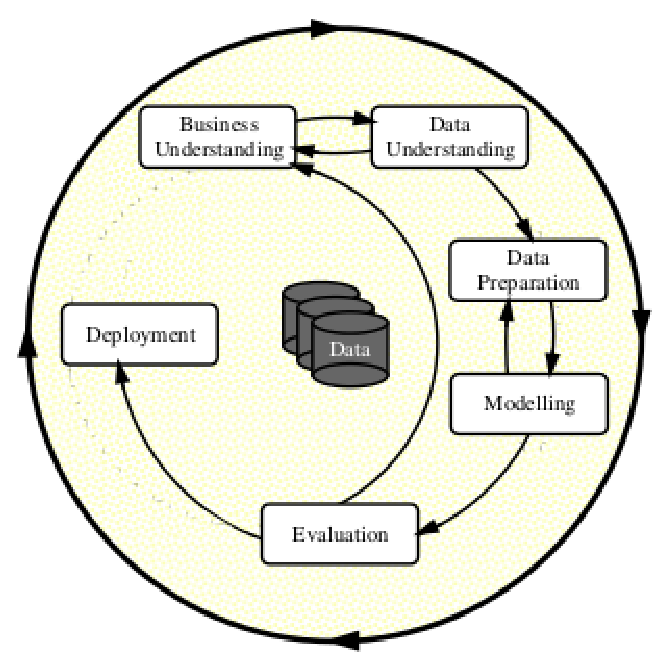
\includegraphics[scale=0.75]{crispdm.eps}
					
		\caption{CRISP-DM \cite{wirth2000crisp} cycle}
		\label{fig:crispdm}

	\end{figure}
	This section has some theory, to get a view of the big picture. Cross Industry Standard Process for Data Mining \cite{wirth2000crisp} is invented out of necessity for better planning, documentation and communication for Data Mining projects. It is divided in multiple phases, as seen in Figure~\ref{fig:crispdm}. The business understanding phase is to describe the urge and the goal of the project, see Section~\ref{seq:motivation}. The data understanding phase is to learn about the data, what is the source and how it is computed. In Section~\ref{sec:sensorsystems},~\ref{sec:datadescription} and ~\ref{sec:bvsb} the sensors systems are described, how they are used and what the data is. Normally the data is already collected, but this project needs another phase. The data collection phase is described in Section~\ref{sec:datacollection}. The next phase is the data preparation phase. In this project it exists out of two parts. The first part is about preprocessing to compute the dataset, as seen in Section~\ref{sec:preprocessing}. The dataset can be used by the Liacs Data Mining Group for further research. The second part is the feature extraction section, which describes the computing of the training set, seen in Section~\ref{sec:feature}. 
	A model is a generalised representation of the data. An algorithm tries to make relations between attributes. There are three reasons to make such an model:
	\begin{enumerate}
		\item Prediction. A bank give loans to clients and they will try to choose the best interest rate, such that the client will accept the interest rate, can pay the interest rate and the loan back over time and the bank will make a profit. Based on data from old clients a model can be made and the probability of a client getting problems with paying the intereset rate can be calculated. Based on this information the high of the loan and the interest rate can be determined \cite{credit}. Another example is predicting the age of a Twitter user \cite{tweetgenie}.		
		\item Insight. After analyzing the correlation between products bought together in a supermarket, management decided to place diapers and beer close together. More customers who bought the diapers were tempted to buy beer just by seeing it, which resulted in more impulsive sales \cite{beer}.
		\item Classification. Email spam (unwanted email) filters are using classification to determine if an e-mail is spam or ham (not spam). Based on the previous received emails with their associated label spam or ham, a model can be made to predict the class of a new received email. 
	\end{enumerate}
	Models need to be trained, by a training set. The bigger the training set, the better the model, because of the chance is higher the set will represent all possible data. The better the model, the better the relations between the attributes are expressed. Section~\ref{sec:classification} analyzes the data by looking to the correlations / explains how to make a model. When the model is made itis time to analyze the results. / Is it possible to achieve the goal? The deployment is the implementation to achieve the goal. This could be a new piece of software for bank employees or a new price for a product. 

	\subsection{Classification}
	\label{sec:classification}
	In this section a model is built of the locations based on the data of the BioHarness and the OpenBeacon. The dataset from Section~\ref{sec:rawdataset}  is used, with some alterations. The nights are removed, because the BioHarness does not measure in the night. The rows with missing values are also removed. This gives us a dataset with more than 585000 instances or rows. WeKa \cite{weka} is a software program with a lot of data mining algorithms included and is used to make the model. The used algorithm is J48 and is an implementation of the C4.5 \cite{quinlan1993c4} decision tree algorithm. 66\% is used as training set and 34\% as validation set. Leafes with less than 10000 instances are removed. This will result in a pruned tree and will prevent overfitting. As a result of the actions to prevent overfitting, the percentage correctly classified instances is only 70\%, despite the large amount of instances. Only the locations ``out'', ``bedroom'' and ``rest of the house'' are classified, because those are most visited as seen in Figure~\ref{fig:histogram}. The tree is still big with 35 leafes. In this setup the data of the BioHarness could only explain some regular visited locations. It could be improved by stratifying sampling. This means the same amount of instances are used of every location, but this will make the model less realistic. It could also be improved by using more specific locations, for instead of the general ``out of the house'' location. I could do all kind of activies out of the house, which also applies for rest of the locations. An other solution could be the use of a lower sampling frequency, like $\frac{1}{60}$ \SI{}{\hertz} (every minute) instead of \SI{1}{\hertz} (every second). See Figure~\ref{fig:classtree} for the decision tree. \\
	The model is built again, because not all the locations showed up in the desicion tree. The difference is this time the three will be pruned less. Leafes with less than 1000 instances are removed. This results in a larger tree, a higher percentage correctly classified instances and more locations will show up in the tree.


	
	\begin{figure}[h]
		\label{fig:classtree}	
		\centering
		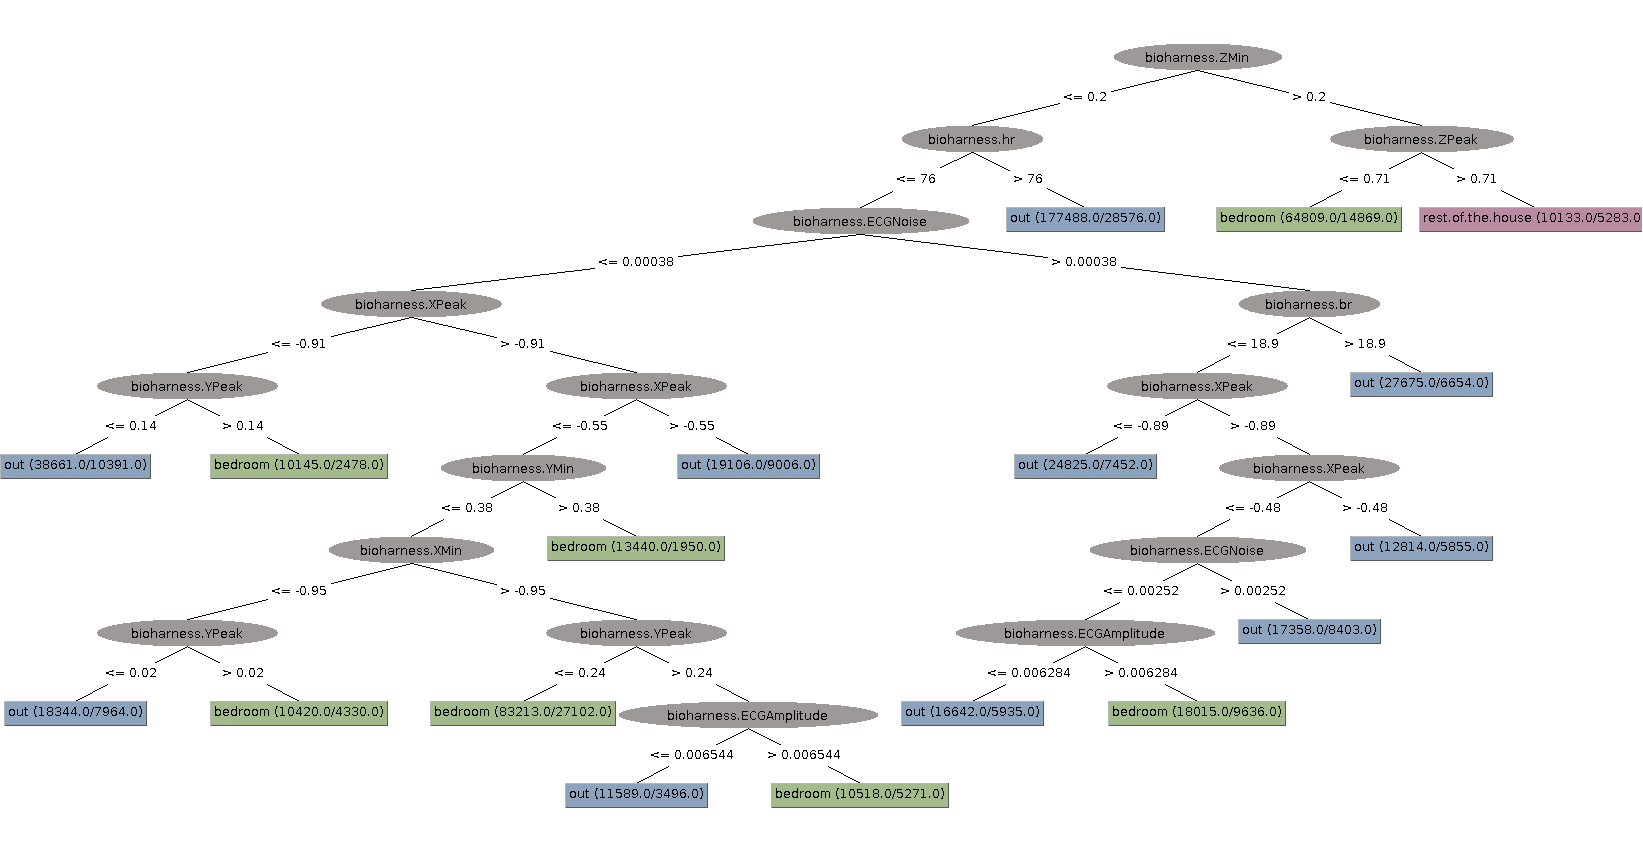
\includegraphics[scale=0.40, angle=90]{tree/edited.png}
		\caption{A decision tree of the first model.}
	\end{figure}


	\iffalse
	\subsection{WeKa}
	- What is WeKa. java implementation for a lot of data mining algorithms.
	- M5p, Quinlan's M5
	- linear regression
	- neural network
	- results 

	avgHr vs hr100+
	out vs bedroom
	out vs hr120-140
	dining.room - kitchen

	inbed vs avgNoise: hoe later naar bed -> hoe minder geluid?, doordat je waarschijnlijk niet aanwezig bent in de kamer.
	outbed vs stageA: later naar bed, vaker away, later opstaan.
	outbed vs inbed: correlatie is 0.21. 

	light sleep neemt toe naarmate ik later naar bed ga, maar deep sleep ook. Val dus sneller in slaap. 
	Sleep efficiency neemt toe als ik latar naar bed ga. (r=0.5) Later opstaan zorgt juist voor het tegenovergestelde.
	later naar bed gaan dan gisteren resulteert ook in lagere sleep efficiency
	outbed vs inbed: r = 0.49
	Sta ik later naar bed, of later uit bed dan gisteren, gaat de efficiency omlaag 
	target

	\newpage
	\fi
	\subsection{Correlations}
	In Table \ref{tab:cor}, 28 correlations are listed. These correlations are based on the dataset produced in Section~\ref{sec:feature}. Analyzing the results gives some trivial conclusions, but also interesting ones. \#3 says when I wake up later, the difference between the previous wake up is greater. The higher the correlations the more consistent the sleep rythm. \#6 says, the later I go to bed, the more I am away from my bed. \#11 is also trivial. \#1 and \#4 are more interesting, because it means when I diverge from my normal sleep rythm, I will sleep less efficient. Going later to bed and waking up later will result\footnote{``Will result'' is not precisely true. Correlation does not mean causality, but in this paragraph the causalities are assumed.}  in less REM sleep and it will not be at the expense of deep sleep. As a matter of fact, the correlation is positive, it will result in a bit more deep and light sleep. Going later to bed will result in less time awake in bed, but sleeping longer in the morning will result in more awake time. \#18 is also an interesting correlation, but the resting heart rate is relative constant, so it does not need to mean anything. A high heart rate will result in a less efficient sleep, based on \#20 and \#27, but based on \#21 and \#24 it will result in more deep sleep. Most trivial correlation is \#28, because stageW is part of the formula to calculate the sleep efficiency.
		

	\clearpage
	\begin{table}
		\centering
		\newcounter{rownum}
		\setcounter{rownum}{0}
		\newcommand\rownumber{\stepcounter{rownum}\arabic{rownum}}
	\begin{tabular}{| c | l | l | l |}
		\hline
		\# & Feature A & Feature B & Correlation \\ \hline
		\rownumber & outbed.difference\tablefootnote{The amount of minutes woke up later than the previous day} & sleep.efficiency\tablefootnote{Relative time slept in bed} & -0.51 \\
		\rownumber & outbed\tablefootnote{Amount of minutes woke up after 08:00 am} & inbed.difference & 0.33 \\
		\rownumber & outbed & outbed.difference & 0.54 \\
		\rownumber & inbed.difference & sleep.efficiency & -0.14 \\
		\rownumber & inbed\tablefootnote{Amount of minutes going to bed after 22:00 pm} & outbed & 0.21 \\ 
		\rownumber & inbed & stageA\tablefootnote{Away} & 0.50 \\
		\rownumber & inbed & stageW\tablefootnote{Wake} & -0.53 \\
		\rownumber & inbed & stageD\tablefootnote{Deep sleep} & 0.10 \\
		\rownumber & inbed & stageL\tablefootnote{Light sleep} & 0.09 \\
		\rownumber & inbed & stageR\tablefootnote{REM sleep} & -0.40 \\
		\rownumber & outbed & stageA & -0.74 \\    
		\rownumber & outbed & stageW & 0.13 \\    
		\rownumber & outbed & stageL & 0.07 \\
		\rownumber & outbed & stageD & 0.03 \\
		\rownumber & outbed & stageR & -0.67 \\
		\rownumber & hr100+ & resting.heartrate & 0.28 \\
		\rownumber & stress.percent & resting.heartrate & -0.35 \\
		\rownumber & out\tablefootnote{Out of the house} & resting.heartrate & 0.65 \\
		\rownumber & stageD & resting.heartrate & -0.15 \\
		\rownumber & hr140+ & sleep.efficiency & -0.59 \\
		\rownumber & hr100+ & stageD & 0.25 \\
		\rownumber & hr100+ & stageL & -0.13 \\
		\rownumber & hr100+ & stageR & -0.41 \\
		\rownumber & avgHR & stageD & 0.32 \\
		\rownumber & avgHR & stageL & -0.17 \\
		\rownumber & avgHR & stageR & -0.46 \\
		\rownumber & avgHR & sleep.efficiency & -0.39 \\
		\rownumber & stageW & sleep.efficiency & -0.99 \\

		\hline
	\end{tabular}
	\caption{A few correlations between different features}
	\label{tab:cor}
	\end{table}
	

	\iffalse

	Business understanding: formulate a goal, what to improve, section 1.2 / 1.3
	Data understanding, What are the systems measuring : Section 2.
	Normally data is already collected, in this project not. So an extra step.
	Data preparation is getting from the raw data to the training set, but in this project there are to steps to produce it.
	First from the raw to the dataset. This dataset can is provided and can be used by the liacs data mining group.
	from dataset to trainingset, in feature extractin section



	Derivate a dataset, use WeKa for modeling, find patterns.

	
	model, A way to describe the data. Generalization.
	prediction, classification, understanding the model.
	- linear regression
	- nearal network
	Now the modeling part.

	Next is the evaluation, which conclusions could be made.

	At least the deployment, implementation of the conclusions. To reach the goal and improvement. 
	\fi

\section{Conclusions}
	Working with the three devices is doable for two weeks, but it takes effort to stay focussed and to not forget anything. With more than a million records from multiple data devices, preprocessing takes a lot of time. The code is not advanced, but it is complex because of all the stages the data needs to go through. A lot of loops are used. The way I used the dataset resulted in a trainingset of 15 days and 15 days is not enough to draw trustworthy conclusions, but it is a begin. There are other ways to use the data and if a sampling frequecy of once per every hour is used, it will give 360 hours. The OpenBeacon is nice to have as an extra, but in my situation location can't explain the things I do, because I use the locations for multiple things and most of the time I'm in my bedroom. 
	There are more interesting subjects than me for the experiment. I live structural, don't have health complains, don't smoke, don't do drugs, drink no or little alcohol, drink no coffee and sport a lot. Not a typical student. When a subject is chosen with an unregular live schedule the correlations between the different features could be different, because relations could be more visible. Before the experiment I was thinking about doing something different in one week and doing something else in the other week. It would be interesting to see how I would react. For example drinking coffee before going to bed. However, data mining has a paradigm to don't use hypotheses. If there is a correlation, it will show up eventually.
	\
	Despite the few days of data, I could agree with the correlations measered. Going later to bed and wake later up will result in more deep sleep, more light sleep and less REM sleep. Based on this I would advice myself to sleep less. With an average of 9 hours and 24 minutes in bed per night, I think that's fair. The interface of Beddit is easy in use and also informative. An advice I read on the website of Beddit was to sleep more structural, even more structural I already did. Now I'm trying to wake up and go to bed every day on the same moment. Beddit is still running at the time of writing this and I visit the website of Beddit still every day. The statistics motivates me to keep me to my schedule and to improve my life style. I changed my environment to make it darker and sometimes uses earplugs to ignore noise. 
	\
	In the further more devices could be added to the experiment. Like the Nike Fuel, easier to wear 24/7. Or something what keeps record on a convient way what I eat, because that's also an really important factor in life. 
	

	In 3-5 years more and more wearable sensors systems are going to be used by the mainstream. Nike already started the mainstream trend with the Nike Fuel stapperteller. They make it comperable and it would be cool to compare yourself with a sport athelete or just a friend. I see it in front of me, "Hé , you ate last week x calories, but sported just 5 hours, prepare yourself Summer is coming." You will challenge each other to sport. 

	Most of the systems will get an API and I predict an online social community will be get popular. It will collect all the data and will make it comparable and sharable with friends. 
	websites / communities will come up to combining the data and present it on a gemakkelijk manier. When that time will come it would be interessant to ask for the data and do data mining experiments again. 

	\iffalse
	preprocessing a lot of time, 
	need more devices, like calories counter or nike feul.
	More interesting subjects, I'm quite boring, I live to structural.
	Sleep in a structured way improve sleep, 
		but not enough data to really proof correlation between day and night
	Interessted future research, find to partners as subject and see how their lives influence each other.
	This is just a basic experiment and could be really extended by a next student.
	15 days is not enough, more like 15 months. 
	naieve about the data. 
	Still, it is a good setup and could be extended and replaced with maybe easier and better sensors. 
 The models didn't work out well.


	- products dataset
	- lot of data
	-  some insides of sleep
	I have bradycardia. 
	- more features for training set, but not enough rows. ratios.

	at first I had a idea to drink before going to bed coffee one week, and the next week no coffee. This will result in hopefully a good different sleep patterns. But the Data Mining has a paradigm to don't stel op a thesis and collect all the data and see the conclusions afterwards. The problem is, I don't drink coffee, much alcohol, drugs, energy drink or strange things that's could give interessant data because it will interupt/aanpassen my normal life. 
When humans query data we start with an idea, such as: "I think that we sell more DVDs to males than to females." And then we run a query to test the idea and the answer either confirms or disproves our hypothesis. A data mining algorithm doesn't have ideas. It has no intention of testing ideas for the simple reason that it doesn't have any.

	For another person who has regular shifts maybe better results would came up.


	The beddid is still running every night, and I watch the resuls every day. I improved my life style, not per se because of this project with combining data, but only to watch the statistiscs of my night and watch the advices it's given me. Yesterday I broke my record of deep sleep at the night. I sleep strictly regular, (yes more regular than during the tracking with the bioharness and the openbeacon combined.) and changed some things in my bedroom to make it darker. I also use more noise cancceling earplugs. So it's interessting just by seeing the data makes me want to improve my lifestyle. 

	Quantified jan is a selftracking freak an has a lot of systems, and he putted it all only. Only it are all sepered systems and not combinbed.

	In 3-5 years more and more wearable sensors systems are going to be used by the mainstream. Nike already started the mainstream trend with the Nike Fuel stapperteller. They make it comperable and it would be cool to compare yourself with a sport athelete or just a friend. I see it in front of me, "Hé , you ate last week x calories, but sported just 5 hours, prepare yourself Summer is coming." You will challenge each other to sport. 

	Most of the systems will get an API and websites / communities will come up to combining the data and present it on a gemakkelijk manier. When that time will come it would be interessant to ask for the data and do data mining experiments again. 


	There are some correlations, but not strong ones. Not much more days to be certain about the correlation.
	\fi


\printbibliography

\end{document}
